% ══════════════════════════════════════════════════════════════════
\chapter{Attempting to Fix the Trap}
\label{ch:fixing_trap}
% ══════════════════════════════════════════════════════════════════

Chapter~\ref{ch:gradient_trap} established that row centering creates a
locked forward/backward gain ratio of $\sqrt{(\pi-1)/\pi} \approx 0.827$.
This chapter explores two strategies to mitigate the resulting gradient
non-uniformity.

% ──────────────────────────────────────────────────────────────────
\section{Partial Centering (Alpha Sweep)}
\label{sec:alpha_sweep}

\subsection{Definition}

For $\alpha \in [0,1]$, define partial centering:
\begin{equation}\label{eq:partial_centering}
  W_{ij} = W_{ij}^{(\mathrm{He})}
           - \alpha \cdot \bar{w}_i,
  \qquad
  \bar{w}_i = \frac{1}{d}\sum_k W_{ik}^{(\mathrm{He})},
\end{equation}
followed by rescaling each row to restore He variance.
At $\alpha = 0$ this is pure He; at $\alpha = 1$ this is full row
centering.

\subsection{Effect on forward gain}

Partial centering with parameter $\alpha$ suppresses a fraction of the
DC component.  The effective input energy seen by the neuron is
approximately:
\begin{equation}
  E_{\mathrm{eff}} \approx \E[a^2] - \alpha^2 \cdot (\E[a])^2
  = \E[a^2]\left(1 - \frac{\alpha^2}{\pi}\right),
\end{equation}
giving forward gain approximately:
\begin{equation}\label{eq:partial_fwd}
  g_{\mathrm{fwd}}(\alpha) \approx \sqrt{1 - \frac{\alpha^2}{\pi}}
  \approx 1 - \frac{\alpha^2}{2\pi}.
\end{equation}
A simpler linear approximation from the data:
$g_{\mathrm{fwd}}(\alpha) \approx 1 - 0.174\,\alpha$.

\subsection{Empirical results}

\textbf{Setup:} 50 hidden layers, width 784, Fashion-MNIST.
PCA geometry metric (used before the k-NN transition; see
Chapter~\ref{ch:geometry} for why this is misleading).

\begin{center}
\begin{tabular}{ccccc}
\toprule
$\alpha$ & Med fwd gain & Med bwd gain & Grad spread & Geometry (PCA) \\
\midrule
0.0 & 0.996 & 0.997 & $6.6\times$ & 0.955 \\
0.2 & 0.937 & 0.996 & $2.4\times$ & 0.905 \\
0.4 & 0.887 & 0.999 & $36.8\times$ & 0.835 \\
0.6 & 0.853 & 0.998 & $294.7\times$ & 0.822 \\
0.8 & 0.832 & 0.999 & $1{,}219\times$ & 0.808 \\
1.0 & 0.826 & 0.999 & $1{,}908\times$ & 0.818 \\
\bottomrule
\end{tabular}
\end{center}

Key observations:
\begin{enumerate}
  \item \textbf{Backward gain $\approx 1.0$ for all $\alpha$:}
        The backward pass is robust to partial centering because the
        transposed weights interact with error signals that have
        near-zero mean.
  \item \textbf{Gradient spread grows exponentially with $\alpha$:}
        Even $\alpha = 0.5$ gives $g_{\mathrm{fwd}} \approx 0.913$,
        which over 50 layers compounds to $0.913^{50} \approx 0.010$
        --- three orders of magnitude decay.
  \item \textbf{No $\alpha$ gives both good gradients and good geometry:}
        $\alpha = 0.2$ minimizes gradient spread ($2.4\times$) but has
        poor geometry.  $\alpha \geq 0.6$ gives good geometry but
        gradient spreads $> 300\times$.
\end{enumerate}

\begin{figure}[h]
\centering
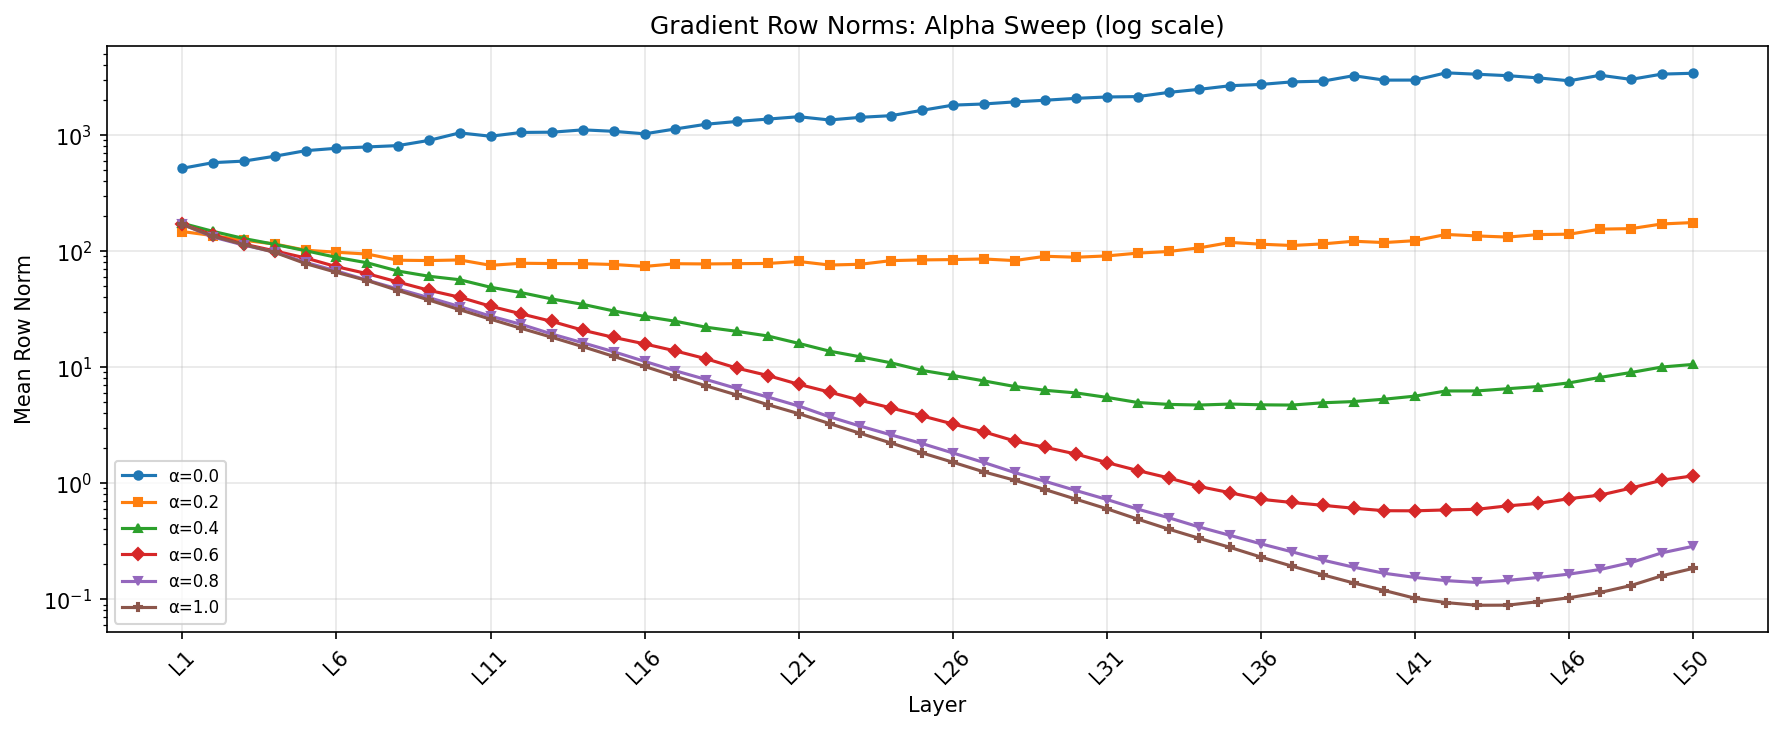
\includegraphics[width=0.85\textwidth]{figures/gradient_norms_alpha_sweep.png}
\caption{Gradient row norms (log scale) across 50 layers for partial centering
  with $\alpha \in \{0, 0.2, 0.4, 0.6, 0.8, 1.0\}$.
  At $\alpha = 0$ (He), gradients are nearly flat.
  At $\alpha = 1$ (full centering), gradients span $\sim\!4$ orders of magnitude.
  Source: \texttt{notebooks/06\_gradient\_diagnostics.ipynb}, Cell~20.}
\label{fig:gradient_norms_alpha}
\end{figure}

\subsection{Conclusion}

Partial centering defines a \textbf{Pareto frontier} between geometry
and gradient uniformity.  It allows choosing \emph{where} on the
trade-off to sit, but cannot escape it.  Any $\alpha$ large enough to
meaningfully suppress DC drift creates enough forward signal loss to
produce non-uniform gradients.

% ──────────────────────────────────────────────────────────────────
\section{Layer-Balanced Initialization (Eta Sweep)}
\label{sec:eta_sweep}

\subsection{Motivation}

The partial centering approach tried to reduce the centering
parameter.  The layer-balanced approach takes a fundamentally different
strategy: \textbf{keep full row centering ($\alpha = 1$) for best
geometry, but use different weight variances at each layer to equalize
gradients despite the forward decay.}

\subsection{Mathematical derivation}

Let each layer $l \in \{1,\dots,L\}$ have weight standard deviation
$s_l$.  From the backpropagation equations:

\textbf{Forward chain} (activation magnitude at layer $l-1$):
\begin{equation}\label{eq:fwd_chain}
  \|\bm{a}^{(l-1)}\| \propto \prod_{k=1}^{l-1} (r \cdot s_k),
\end{equation}
where $r = \sqrt{(\pi-1)/\pi} \approx 0.826$ is the structural
centering loss per layer, and $r \cdot s_k$ is the forward amplitude
gain at layer~$k$.

\textbf{Backward chain} (error signal at layer $l$):
\begin{equation}\label{eq:bwd_chain}
  \|\bm{\delta}^{(l)}\| \propto \prod_{k=l+1}^{L} s_k.
\end{equation}
The backward gain at layer~$k$ is approximately $s_k$ (Section~\ref{sec:bwd_gain}).

\textbf{Gradient at layer $l$} (from BP4, equation~\eqref{eq:bp4}):
\begin{equation}\label{eq:grad_layer}
  \left\|\frac{\partial \mathcal{C}}{\partial W^{(l)}}\right\|
  \propto \|\bm{a}^{(l-1)}\| \cdot \|\bm{\delta}^{(l)}\|
  \propto \prod_{k=1}^{l-1}(r \cdot s_k) \cdot \prod_{k=l+1}^{L} s_k
  = r^{l-1} \cdot \frac{\prod_{k=1}^{L} s_k}{s_l}.
\end{equation}

Since $\prod_{k=1}^{L} s_k$ is a constant (independent of $l$),
the gradient depends on $l$ only through:
\begin{equation}\label{eq:grad_prop}
  \left\|\frac{\partial \mathcal{C}}{\partial W^{(l)}}\right\|
  \propto \frac{r^{l-1}}{s_l}.
\end{equation}

\textbf{For uniform gradients}, we need $r^{l-1}/s_l = \text{const}$,
which gives:
\begin{equation}\label{eq:optimal_sl}
  s_l \propto r^{l-1}.
\end{equation}

Early layers ($l$ small) get $s_l$ large (boosted weights);
late layers ($l$ large) get $s_l$ small (reduced weights).

\subsection{Parameterization}

We center the scaling at the middle layer and introduce a strength
parameter $\eta$:
\begin{equation}\label{eq:sl_param}
  s_l = r^{\,\eta \cdot (l - (L+1)/2)},
\end{equation}
so that $s_{(L+1)/2} = 1$ (middle layer unchanged).

\begin{itemize}
  \item $\eta = 0$: $s_l = 1$ for all $l$ (no correction).
  \item $\eta = 1$: full correction ($s_l = r^{l-(L+1)/2}$).
  \item $\eta = 0.5$: half correction.
\end{itemize}

The total weight std at layer $l$ is
$\sigma_l = \sigma_{\mathrm{base}} \cdot s_l$, where
$\sigma_{\mathrm{base}} = \sqrt{2/d} \cdot \sqrt{\pi/(\pi-1)}$
is the forward-balanced base (see the flag in
Section~\ref{sec:layer_balanced}).

\subsection{Results}

\textbf{Setup:} 20 hidden layers, width 784, Fashion-MNIST.

\begin{center}
\begin{tabular}{ccccc}
\toprule
Config & Grad ratio & Grad CV & Med fwd gain & Med bwd gain \\
\midrule
He (baseline) & $1.93\times$ & 0.182 & 0.979 & 1.022 \\
$\eta = 0.00$ & $11.41\times$ & 0.926 & 0.999 & 1.213 \\
$\eta = 0.25$ & $6.52\times$ & 0.603 & 1.045 & 1.212 \\
$\bm{\eta = 0.50}$ & $\bm{4.32\times}$ & \textbf{0.521} & 1.096 & 1.212 \\
$\eta = 0.75$ & $6.67\times$ & 0.764 & 1.150 & 1.212 \\
$\eta = 1.00$ & $12.93\times$ & 1.075 & 1.206 & 1.212 \\
\bottomrule
\end{tabular}
\end{center}

\begin{flagbox}
At $\eta = 0$, the median forward gain is $0.999$ and the backward
gain is $1.213$.  This means $\eta = 0$ corresponds to the
\textbf{forward-balanced} base (Section~\ref{sec:rc_fwd_balanced}),
\emph{not} the variance-adjusted base (which would give forward
gain $\approx 0.826$ and backward gain $\approx 1.0$).
\end{flagbox}

\subsection{Analysis}

\begin{enumerate}
  \item \textbf{$\eta = 0.5$ is the sweet spot:}
        Gradient ratio improves from $11.41\times$ to $4.32\times$
        ($\sim 2.6\times$ improvement), CV from 0.926 to 0.521.
        Still worse than He's $1.93\times$.

  \item \textbf{$\eta = 1.0$ is worse than $\eta = 0$:}
        Gradient ratio $12.93\times$ vs.\ $11.41\times$.
        The full correction \textbf{overshoots}.

  \item \textbf{Backward gain is $1.21$ for ALL $\eta$:}
        The backward gain depends on the average weight scale
        (the forward-balanced base), not on how variance is
        distributed across layers.
        Over 20 layers: $1.21^{20} \approx 55\times$ backward
        amplification.
\end{enumerate}

\begin{figure}[h]
\centering
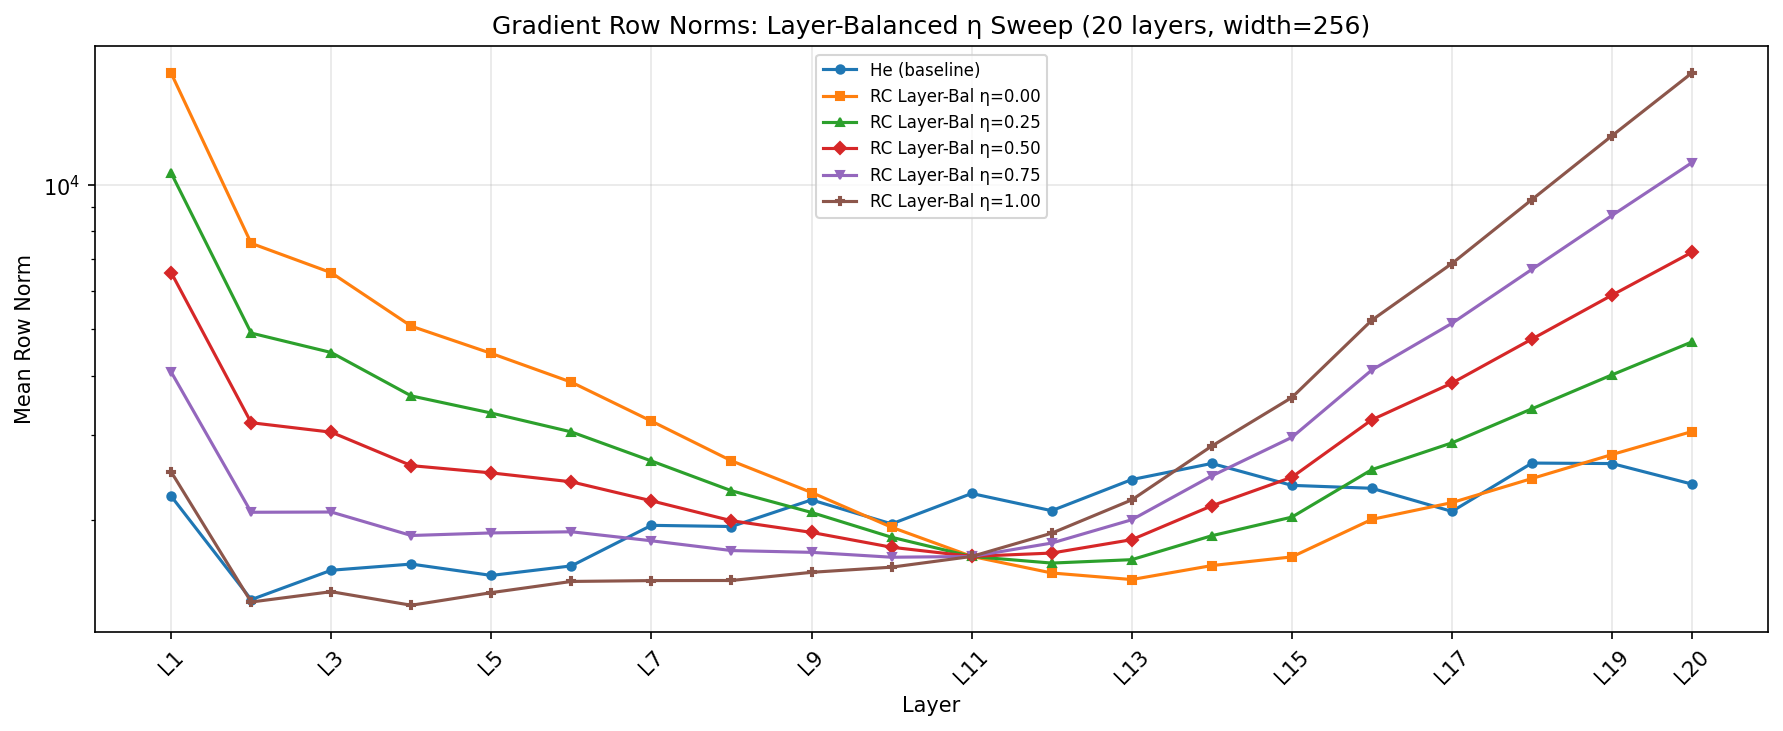
\includegraphics[width=0.85\textwidth]{figures/gradient_norms_eta_sweep.png}
\caption{Gradient row norms (log scale) for layer-balanced initialization
  with $\eta \in \{0, 0.25, 0.5, 0.75, 1.0\}$ and He baseline.
  $\eta = 0.5$ achieves the flattest profile among row-centered variants.
  Source: \texttt{notebooks/06\_gradient\_diagnostics.ipynb}, Cell~23.}
\label{fig:gradient_norms_eta}
\end{figure}

\subsection{Why $\eta = 1$ overshoots}

At $\eta = 1$, the per-layer scaling
$s_l = r^{l - (L+1)/2}$ fully compensates forward decay.
But it also makes the backward gain \textbf{non-uniform}:

\begin{itemize}
  \item Early layers: $s_l > 1$ (boosted weights) $\Rightarrow$
        backward gain $= 1.21 \times s_l \gg 1$
        (up to ${\sim}7$ in the empirical plot).
  \item Late layers: $s_l < 1$ (reduced weights) $\Rightarrow$
        backward gain $= 1.21 \times s_l < 1$.
\end{itemize}

The layer-dependent $s_l$ that fixes the forward chain
\textbf{destabilizes the backward chain}.
At $\eta = 0.5$, the partial compensation balances forward improvement
against backward destabilization.

\subsection{Comparison to partial centering}

\begin{center}
\begin{tabular}{lccc}
\toprule
Approach & Gradient spread & Geometry & Mechanism \\
\midrule
Partial centering ($\alpha = 0.25$) & $6.6\times$ & Poor & Reduce centering \\
Layer-balanced ($\eta = 0.5$) & $4.32\times$ & Best (full RC) & Redistribute variance \\
\bottomrule
\end{tabular}
\end{center}

The layer-balanced approach is \textbf{strictly better on the Pareto
frontier}: it achieves lower gradient spread ($4.32\times$ vs.\
$6.6\times$) while maintaining full row-centered geometry.

\subsection{Fundamental limitation}

The backward gain of $1.21$ (from the forward-balanced base) limits
how much the layer-balanced approach can improve.
The $\eta$ parameter redistributes gradient non-uniformity between
forward and backward chains but cannot eliminate it.
The optimal $\eta \approx 0.5$ represents the point where forward
compensation and backward destabilization are balanced.
